\section{单纯上同调群}
\sourcepage{308}
本节定义单纯复形的上同调群，并计算一些初等例子。

\entry{定义}{5.3.1}设 $K$ 为单纯复形，$G$ 为阿贝尔群。以 $G$ 为系数的 $p$ 维\textbf{上链群}（cochain group）为
\[
C^p(K;G)=\operatorname{Hom}(C_p(K),G).
\]
\textbf{上边缘算子}（coboundary operator）$\delta:C^p(K;G)\to C^{p+1}(K;G)$ 是边缘算子 $\partial:C_{p+1}(K)\to C_p(K)$ 的对偶，因此使维数升高一维。记其核为\textbf{上闭链群} $Z^p(K;G)$，像为\textbf{上边缘群} $B^{p+1}(K;G)$。由 $\partial^2=0$ 得 $\delta^2=0$，于是定义\textbf{上同调群}
\[
H^p(K;G)=Z^p(K;G)/B^p(K;G).
\]
若系数为整数，通常省略 $G$。

\sourcepage{309}
对于上链 $c^p$ 与链 $c_p$，通常用对偶配对 $\langle c^p,c_p\rangle$ 表示上链在链上的取值。此时上边缘的定义为
\[
\langle\delta c^p,d_{p+1}\rangle=\langle c^p,\partial d_{p+1}\rangle.
\]
这个定义确实很代数化，但仍可在一定程度上作几何理解。

任意为 $K$ 的 $p$ 维单形定向，得到 $C_p(K)$ 的自由基 $\{\sigma_\alpha\}$。链必须是有限和 $\sum n_\alpha\sigma_\alpha$；上链则由它在每个基元上的值 $g_\alpha\in G$ 唯一决定，这些值可以任意指定，不要求仅有限个非零。

令整数\textbf{初等上链} $\sigma_\alpha^*$ 在 $\sigma_\alpha$ 上取 $1$，在其余基元上取 $0$。对 $g\in G$，用 $g\sigma_\alpha^*$ 表示在该基元上取 $g$、其他处为零的上链。于是可将任意上链写成可能无限的\emph{形式和}
\[
c^p=\sum_\alpha g_\alpha\sigma_\alpha^*.
\]
其依据是：若 $C_\alpha$ 为 $\sigma_\alpha$ 生成的无限循环群，则
\[
C^p(K;G)=\operatorname{Hom}(\bigoplus C_\alpha,G)
\cong\prod_\alpha\operatorname{Hom}(C_\alpha,G).
\]
形式和只是用来替代直积的元组记号。

这种记号在计算上边缘时很方便，且确有
\[
\delta c^p=\sum_\alpha g_\alpha\delta\sigma_\alpha^*.
\]
为验证，对任意有向 $(p+1)$ 维单形 $\tau$，写 $\partial\tau=\sum_{i=0}^{p+1}\epsilon_i\sigma_{\alpha_i}$，$\epsilon_i=\pm1$。于是
\[
\langle\delta c^p,\tau\rangle=\sum_{i=0}^{p+1}\epsilon_i g_{\alpha_i}.
\]
右侧形式和中只有对应这有限个面的项在 $\tau$ 上非零，取值同为此和。因此公式有意义并成立。

\sourcepage{310}
故只需计算初等上链的上边缘：
\[
\delta\sigma^*=\sum_j\epsilon_j\tau_j^*,
\]
其中 $\tau_j$ 遍历所有以 $\sigma$ 为面的 $(p+1)$ 维单形，$\epsilon_j$ 是 $\sigma$ 在 $\partial\tau_j$ 中的符号。对任意单形取值即可验证。下面只作少量计算，一般计算问题留待后面。

\entry{例}{5.3.2}取图 5.3.1 的复形，顶点为 $v_i$，边 $e_i$ 与二维单形 $\sigma_i$ 均按图定向。边 $e_5$ 在 $\partial\sigma_1$、$\partial\sigma_2$ 中的系数分别为 $1,-1$，故
\[
\delta e_5^*=\sigma_1^*-\sigma_2^*.
\]
\begin{center}
\includegraphics[width=.96\textwidth]{figures/5-3-1.pdf}\\图 5.3.1\end{center}
类似地，$\delta v_1^*=e_1^*+e_5^*-e_2^*$。由于无三维单形，$\sigma_1^*,\sigma_2^*$ 均为上闭链；它们也都是上边缘，因为 $\delta e_1^*=-\sigma_1^*$、$\delta e_3^*=-\sigma_2^*$。

\sourcepage{311}
一维上链 $c^1=e_1^*+e_5^*-e_3^*$ 也是上闭链，而且等于 $\delta(v_1^*+v_2^*)$。零维上链 $c^0=v_0^*+v_1^*+v_2^*+v_3^*$ 也是上闭链，但不是上边缘，因为不存在负一维上链。

\entry{定义}{5.3.3}若两个上链之差为上边缘，称它们\textbf{上同调}（cohomologous）。例如上式说明 $\sigma_1^*$ 与 $\sigma_2^*$ 上同调。

\entry{例}{5.3.4}考虑图 5.3.2 中稍简化的环面三角剖分。令
\[
z^1=e_1^*+e_2^*+e_3^*+e_4^*+e_5^*+e_6^*,\qquad
d^1=e_7^*+e_8^*+e_9^*+e_{10}^*+e_{11}^*+e_{12}^*.
\]
它们都是上闭链，而且 $\delta(c^*+h^*+j^*)=z^1-d^1$，所以彼此上同调。
\begin{center}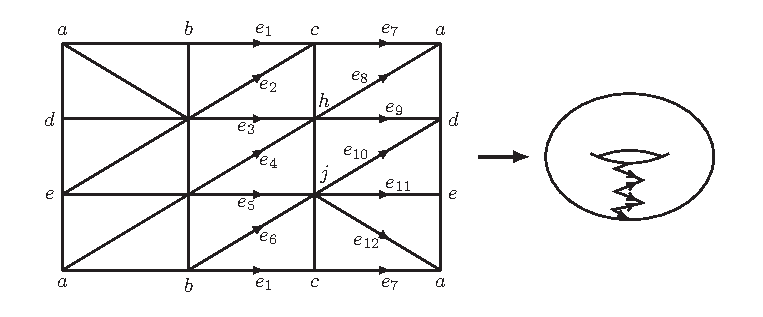
\includegraphics[width=.96\textwidth]{figures/5-3-2.pdf}\\图 5.3.2\end{center}
这说明：一维闭链可以想成闭曲线，而一维上闭链更适合想成一道栅栏！第 5.8 节将证明 $z^1$ 代表 $H^1(T)$ 的一个生成元。

\sourcepage{312}
\entry{例}{5.3.5}计算图 5.3.3 的复形 $K$。一般零维上链为 $c^0=\sum n_iv_i^*$，其上边缘在 $e_1$ 上取 $n_2-n_1$，在 $e_2$ 上取 $n_3-n_2$，依此类推。所以它上闭当且仅当所有 $n_i$ 相等。没有零维上边缘，故 $H^0(K)\cong\Z$，生成元由 $\sum v_i^*$ 代表。
\begin{center}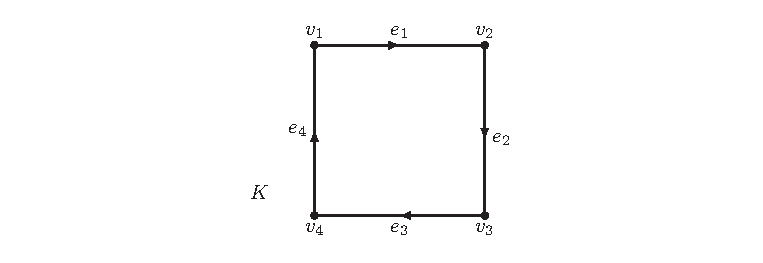
\includegraphics[width=.96\textwidth]{figures/5-3-3.pdf}\\图 5.3.3\end{center}
每个一维上链都上闭。各 $e_i^*$ 都与 $e_1^*$ 上同调，例如 $\delta(v_4^*+v_1^*)=e_3^*-e_1^*$。因此每个一维上链都上同调于 $e_1^*$ 的某个倍数。

这个倍数仅在为零时可能为上边缘：取闭链 $z=e_1+e_2+e_3+e_4$。任意零维上链满足 $\langle\delta c^0,z\rangle=\langle c^0,\partial z\rangle=0$，而 $\langle ne_1^*,z\rangle=n$。所以 $H^1(K)\cong\Z$，由 $e_1^*$ 的类生成，也可由其他任一边的初等上链生成。这一论证同样适用于任意多边形。

\entry{例}{5.3.6}上一例中同调与上同调群相同，下面说明一般并非如此。取图 5.3.4 的 Klein 瓶 $S$。已知 $H_2(S)=0$，但 $H^2(S)$ 非零。

\sourcepage{313}
\begin{center}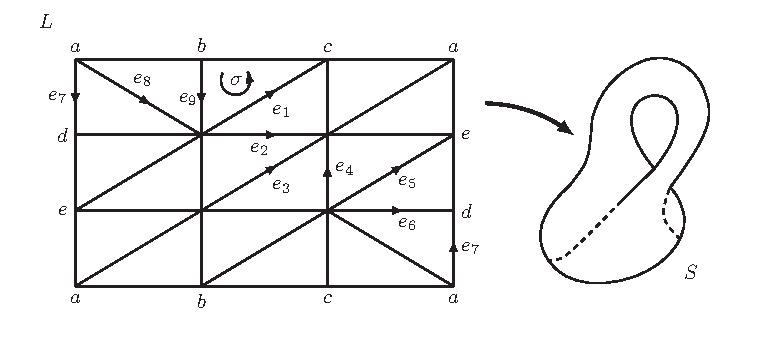
\includegraphics[width=.96\textwidth]{figures/5-3-4.pdf}\\图 5.3.4\end{center}
将矩形 $L$ 的二维单形逆时针定向，并把定向传到 $S$，记其和为 $\gamma$。它不是闭链，因为 $\partial\gamma=2z_1$，其中 $z_1=[a,d]+[d,e]+[e,a]$。

取图中的一个有向二维单形 $\sigma$。因无三维单形，$\sigma^*$ 上闭。对任意一维上链，
\[
\langle\delta c^1,\gamma\rangle=\langle c^1,\partial\gamma\rangle=2\langle c^1,z_1\rangle
\]
为偶数，而 $\langle\sigma^*,\gamma\rangle=1$，故 $\sigma^*$ 不是上边缘。它实际上代表一个二阶元素：可核对图中 $e_1^*+\cdots+e_9^*$ 的上边缘恰为 $2\sigma^*$。

\entry{定理}{5.3.7}$H^0(K;G)$ 等于所有在同一连通分支的顶点上取相同值的零维上链组成的群。特别地，若 $|K|$ 连通，则 $H^0(K)\cong\Z$，生成元是在每个顶点上取值 $1$ 的上链。

\textbf{证明：}没有零维上边缘，所以只需确定零维上闭链。若顶点 $v,w$ 属于同一分支，可取一维链 $c_1$ 使 $\partial c_1=v-w$。对上闭链 $c^0$，
\[
0=\langle\delta c^0,c_1\rangle=\langle c^0,v\rangle-\langle c^0,w\rangle.
\]
反之，若它在同一分支各顶点上相等，则对每条有向边 $\sigma$，$\langle\delta c^0,\sigma\rangle=\langle c^0,\partial\sigma\rangle=0$，所以 $\delta c^0=0$。\hfill$\square$

\sourcepage{314}
因此，$H^0(K)$ 是每个连通分支对应一个 $\Z$ 的直积，而 $H_0(K)$ 是这些群的直和。这又是同调与上同调不同的一个例子。

\entry{定义}{5.3.8}将标准增广 $C_1(K)\xrightarrow{\partial_1}C_0(K)\xrightarrow{\epsilon}\Z$ 对偶化，得
\[
C^1(K;G)\xleftarrow{\delta^1}C^0(K;G)\xleftarrow{\overline\epsilon}G.
\]
称 $\overline\epsilon$ 为\textbf{余增广}（coaugmentation）。它单射，且 $\delta^1\overline\epsilon=0$。定义\textbf{约化上同调}：正维与普通上同调相同，而
\[
\widetilde H^0(K;G)=\ker\delta^1/\operatorname{im}\overline\epsilon.
\]

\entry{定理}{5.3.9}若 $|K|$ 连通，则 $\widetilde H^0(K;G)=0$。更一般地，$H^0(K;G)\cong\widetilde H^0(K;G)\oplus G$。

\textbf{证明：}连通时，增广链列 $C_1(K)\to C_0(K)\to\Z\to0$ 正合，对偶列也正合，所以约化零维上同调为零。其余结论留作习题。\hfill$\square$

\subsection*{习题}
\begin{enumerate}
\item 对例 5.3.2 的复形，求每一维上闭链群的一组基，并证明正维上同调为零。
\item 核对例 5.3.2、定义 5.3.3 附近及例 5.3.4 的计算。\translatornote{原书把 5.3.3 也称为例，实际上它是定义。}
\item \begin{enumerate}[label=(\alph*)]
\item 设 $C_1\xrightarrow{\varphi}C_0\xrightarrow{\epsilon}\Z$ 满足 $\epsilon\varphi=0$，且 $\epsilon$ 满射。考察对偶列，证明 $\operatorname{im}\overline\epsilon$ 是 $\operatorname{Hom}(C_0,G)$ 的直和项，因而也是 $\ker\overline\varphi$ 的直和项。〔见第 1.8 节习题。〕
\item 推出 $\ker\overline\varphi\cong(\ker\overline\varphi/\operatorname{im}\overline\epsilon)\oplus G$，特别地 $H^0(K;G)\cong\widetilde H^0(K;G)\oplus G$。
\end{enumerate}
\item 设 $K$ 的多面体为实数轴，顶点为整数，$\sigma_n=[n,n+1]$。对任意上链 $\sum_{i=-\infty}^{\infty}a_i\sigma_i^*$，显式找一个零维上链以它为上边缘，从而证明 $H^1(K)=0$。
\item 〔*〕设 $K$ 为有限复形。
\begin{enumerate}[label=(\alph*)]
\item 用第 1.12 节链复形标准基定理，以 Betti 数和挠系数表示 $H^p(K)$。
\item 以相同数据表示 $H^p(K;G)$，答案涉及 $G$、$G/mG$ 及乘以 $m$ 的核。
\item 对环面、Klein 瓶、射影空间计算 $H^p(X;G)$。
\end{enumerate}
\item 计算二维球面的上同调。高维球面更难直接计算，为什么？
\end{enumerate}
